% Canonical schema tree — Task 11 deliverable.
% Hand-authored TikZ (it depicts a type structure, not measured data, so there
% is nothing for generate_tables.py to derive). Field names verified against
% src/els_pipeline/models.py: HierarchyLevel{code,name,description};
% NormalizedStandard{standard_id,country,state,version_year,domain,strand?,
% sub_strand?,indicator,age_band?,source_page,source_text}.
\begin{figure}[t]
\centering
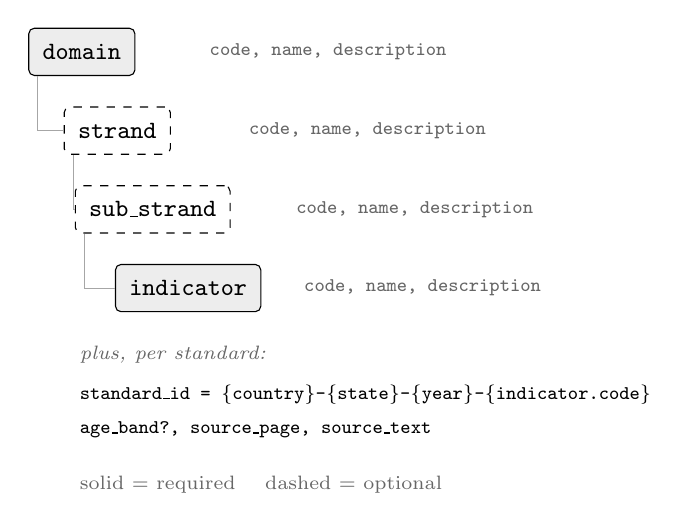
\begin{tikzpicture}[
  font=\small,
  lvl/.style={draw, rounded corners=2pt, minimum height=6mm, inner xsep=5pt, align=left},
  req/.style={lvl, fill=black!7},
  opt/.style={lvl, dashed, fill=white},
  ann/.style={font=\scriptsize\ttfamily, anchor=west, text=black!60},
  link/.style={-, gray!70}
]
\node[req] (d)  at (0,0)      {\texttt{domain}};
\node[opt] (s)  at (0.45,-1)  {\texttt{strand}};
\node[opt] (ss) at (0.90,-2)  {\texttt{sub\_strand}};
\node[req] (i)  at (1.35,-3)  {\texttt{indicator}};

\draw[link] (d.south west) ++(0.12,0) |- (s.west);
\draw[link] (s.south west) ++(0.12,0) |- (ss.west);
\draw[link] (ss.south west) ++(0.12,0) |- (i.west);

\node[ann] at (1.5,0)    {code, name, description};
\node[ann] at (2.0,-1)   {code, name, description};
\node[ann] at (2.6,-2)   {code, name, description};
\node[ann] at (2.7,-3)   {code, name, description};

\node[font=\scriptsize, anchor=west, text=black!60] at (-0.15,-3.85)
  {\textit{plus, per standard:}};
\node[font=\scriptsize\ttfamily, anchor=west] at (-0.15,-4.35)
  {standard\_id = \{country\}-\{state\}-\{year\}-\{indicator.code\}};
\node[font=\scriptsize\ttfamily, anchor=west] at (-0.15,-4.8)
  {age\_band?, source\_page, source\_text};

\node[font=\scriptsize, anchor=west, text=black!60] at (-0.15,-5.5)
  {solid = required \quad dashed = optional};
\end{tikzpicture}
\caption{The canonical schema. Four hierarchy levels, of which
\texttt{strand} and \texttt{sub\_strand} are optional --- Colorado publishes no
sub-strand tier and Texas realizes almost none, so requiring every level would
force the pipeline to invent structure. Each level carries a code, a name and an
optional description. A stored record is one indicator together with its fully
resolved ancestry, not a node in a tree, which is why the identifier embeds the
indicator's already-qualified code and carries any disambiguator itself
(\S\ref{sec:schema}). Every record also retains the source page and the verbatim
text it was extracted from, so any row can be checked against the document that
produced it.}
\label{fig:schema}
\end{figure}
